\label{sec:fetching}
 
Das EEG Headset schickt enkodierte Byte-Sequenzen via Bluetooth, an die proprietären Emotiv Premium Libraries oder die Open-Source Lösung Emotkit (vgl. \ref{chap:eeg}). Die Emokit Klasse wurde für das Projekt leicht modifiziert, sodass sie sich ins System einfügt. So wurde Unterstützung für das neueste EPOC+ Modelle implementiert, sowie die Möglichkeit, Testdaten  aus aus dem TableReader zu versenden. 
Die dekodierten Rohdaten enthalten 14 EEG Kanäle mit Wert und Qualität, die Gyroskopwerte in X- und Y-Richtung und einen Zeitstempel (Abb. \ref{fig:data_processing}). Diese Daten können als CSV gespeichert werden, sowie an einen HTTP-Server oder direkt an den DataCollector übergeben werden. Über den Server integriert die SimToCAN Anwendung via HTTP die EEG Daten in den Fahrsimulator und das virtuelle Steuergerät (\ref{chap:data}).

\begin{figure}[h] 
  \begin{center}
    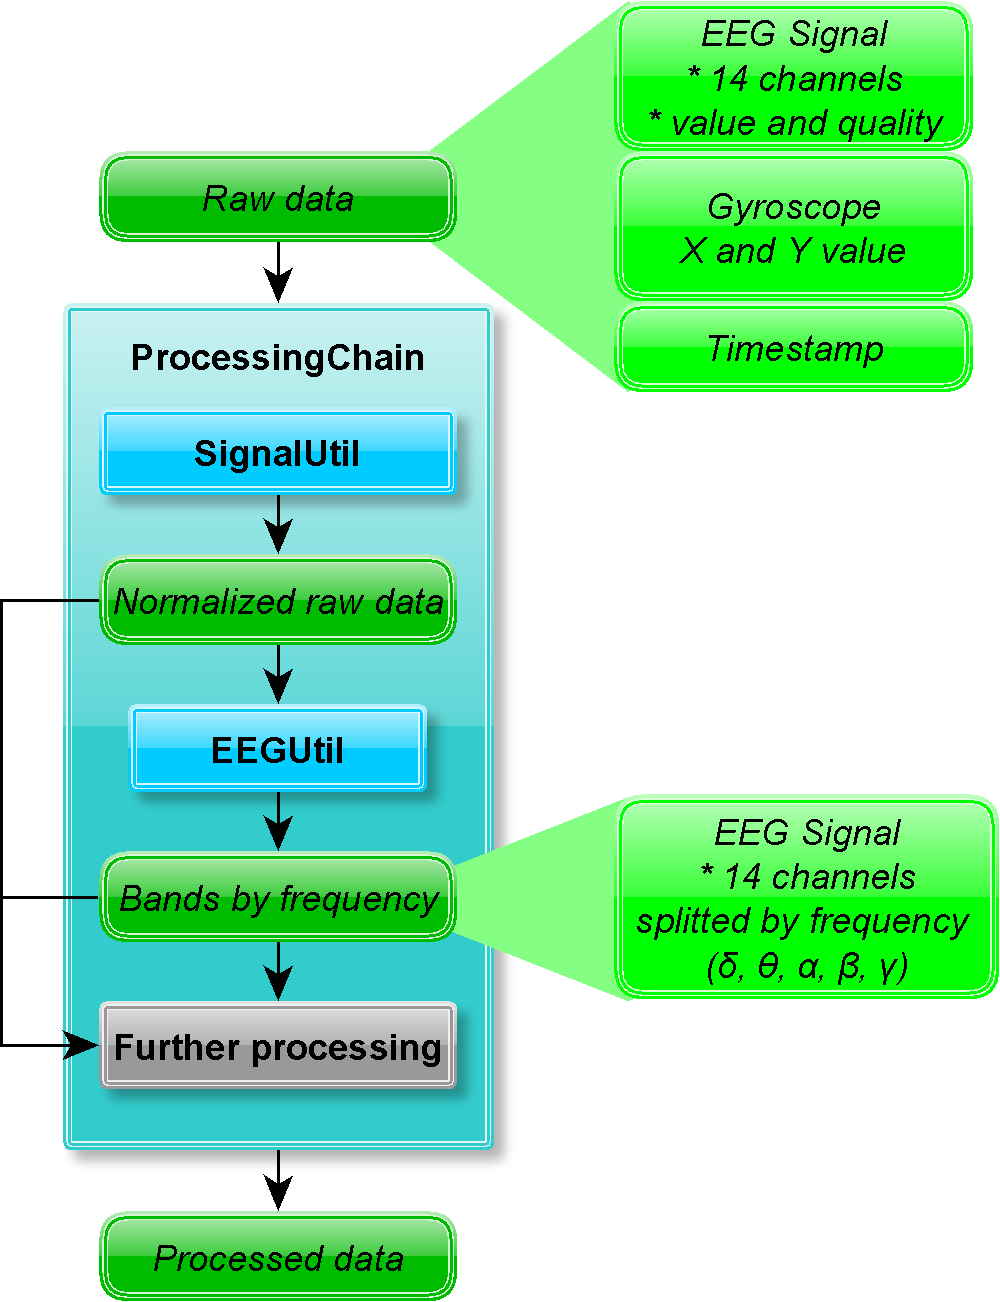
\includegraphics[width=5.5cm]{data_processing}
    \caption[Datenverarbeitung]{Die Daten werden immer weiter reduziert und verarbeitet. \label{fig:data_processing}}
  \end{center}
\end{figure}

Der DataCollector kann Daten direkt oder aus einem HTTP-Client empfangen. Die Schnittstelle zum Fahrsimulator bzw. zum CAR-Interface ist vorbereitet. So ist es möglich die Datensammlung und die Datenverarbeitung auf verschiedenen Rechnern durchzuführen.

Die Aufgabe der DataCollector-Klasse ist es, die einzelnen Signale in Sequenzfenstern von 128 Signalwerten zu aggregieren. Das ist die Abtastrate des EEG-Headsets und entspricht somit in etwa den Signalen einer Sekunde. Es sind zwei dieser Fenster implementiert und sie überschneiden sich in der Hälfte. So ist gewährleistet, dass signifikante Stellen nicht verloren gehen. Die Fensterfunktion ist ein simples Rechteck, sodass alle Werte gleich gewichtet werden. Eine andere Fensterfunktion bspw. mit Glockenkurvenerlauf (Hamming- oder Hann-Fenster) wäre einfach einzubauen. Zudem fügt der DataCollector nur konfigurierte Kanäle hinzu, sodass sich die Datenmenge reduziert. Im folgenden Abschnitt werden die gefilterten Sequenzfenster nun verarbeitet und aufbereitet.
